\documentclass[titlepage, a4paper]{article}
%importerat (2017-01-24) layout-bibliotek från Hannes Snögren, KMM 14/15. Med godkännande från honom. 
%ändrat i settings sedan dess. babel-bibliotek för swedish krävs för kompilering.
%debian: sudo apt-get install texlive-lang-european

\usepackage[swedish]{babel}
\usepackage[utf8]{inputenc}
\usepackage{color}
\usepackage{graphicx}
\usepackage{etoolbox}
\usepackage{hyperref}
\usepackage{calc}  
\usepackage{enumitem}
\usepackage{titlesec}

\makeatletter
\patchcmd{\ttlh@hang}{\parindent\z@}{\parindent\z@\leavevmode}{}{}
\patchcmd{\ttlh@hang}{\noindent}{}{}{}
\makeatother

%Spacing för sections och subsections
\titlespacing*{\section}
{0pt}{5.5ex plus 1ex minus .2ex}{1.0ex plus .2ex}
%\titlespacing*{\subsection}
%{0pt}{5.5ex plus 1ex minus .2ex}{4.3ex plus .2ex}

% Sidformat
\usepackage{a4wide}

% Fixa Appendix-titlar
\usepackage[titletoc,title]{appendix}

% Bättre tabeller
\usepackage{tabularx}

% Bättre bildtexter
\usepackage[margin=10pt,font=small,labelfont=bf,labelsep=endash]{caption}

% Enkelt kommando som låter mig attgöra-markera text
\newcommand{\todo}[1] {\textbf{\textcolor{red}{#1}}}

% Nytt \paragraph låter oss ha onumrerade bitar
\makeatletter
\renewcommand\paragraph{\@startsection{paragraph}{4}{\z@}%
{-3.25ex\@plus -1ex \@minus -.2ex}%
{1.5ex \@plus .2ex}%
{\normalfont\normalsize\bfseries}}
\makeatother

\providecommand{\LAYOUTlogga}{../mall/Logga.png}
\providecommand{\LAYOUTdatum}{\today}


%% Headers och Footers
\usepackage{fancyhdr}
\pagestyle{fancy}
\lhead{\includegraphics[scale=0.12]{\LAYOUTlogga}}
\setlength{\headsep}{0.4in}
\rhead{\ifdef{\LAYOUTutfardare}{Utfärdat av \LAYOUTutfardare \\\LAYOUTdatum}\LAYOUTdatum}
\lfoot{\LAYOUTkursnamn \\ \LAYOUTdokumenttyp}
\cfoot{\thepage}
\rfoot{\LAYOUTprojektgrupp \\ \LAYOUTprojektnamn}

%% Titelsida
\newcommand{\LAYOUTtitelsida}{%
{\ }\vspace{45mm}
\begin{center}
  \textbf{\Huge \LAYOUTdokument}
\end{center}
\begin{center}
  {\Large Redaktör: \LAYOUTredaktor}
\end{center}
\begin{center}
  {\Large \textbf{Version \LAYOUTversion}}
\end{center}
\vspace{5mm}
\ifdef{\LAYOUTfrontpicture}{
\begin{center}
    \LAYOUTfrontpicture
\end{center}
}

\newpage
}


% Projektidentitet
\newenvironment{LAYOUTprojektidentitet}{%
{\ }\vspace{45mm}
\begin{center}
  {\Large PROJEKTIDENTITET}\\[0.5ex]
  {\small
  \LAYOUTartaltermin, \LAYOUTprojektgrupp\\
  Linköpings Tekniska Högskola, IDA
  }
\end{center}
\begin{center}
  {\normalsize Gruppdeltagare}\\
  \def\arraystretch{1.5}%
  \begin{tabular}{|l|l|p{25mm}|l|}
    \hline
    \textbf{Namn} & \textbf{Ansvar} & \textbf{Telefon} & \textbf{E-post} \\
    \hline
}%
{%
    \hline
  \end{tabular}
\end{center}
\begin{center}
  {\small
    \ifdef{\LAYOUTgruppadress}{\textbf{E-postlista för hela gruppen}: \LAYOUTgruppadress\\}{}
    \ifdef{\LAYOUTgrupphemsida}{\textbf{Hemsida}: \LAYOUTgrupphemsida\\[1ex]}{}
    \ifdef{\LAYOUTkund}{\textbf{Kund}: \LAYOUTkund\\}{}
    \ifdef{\LAYOUTkundkontakt}{\textbf{Kontaktperson hos kund}: \LAYOUTkundkontakt\\}{}
    \ifdef{\LAYOUTkursansvarig}{\textbf{Kursansvarig}: \LAYOUTkursansvarig\\}{}
    \ifdef{\LAYOUThandledare}{\textbf{Handledare}: \LAYOUThandledare\\}{}
  }
\end{center}
\newpage
}
\newcommand{\LAYOUTgruppmedlem}[4]{\hline {#1} & {#2} & {#3} & {#4} \\}

%% Dokumenthistorik
\newenvironment{LAYOUTdokumenthistorik}{%
\begin{center}
  Dokumenthistorik\\[1ex]
  %\begin{small}
  \def\arraystretch{1.5}%
    \begin{tabular}{|l|l|p{45mm}|p{30mm}|l|}
      \hline
      \textbf{Version} & \textbf{Datum} & \textbf{Utförda förändringar} & \textbf{Utförda av} & \textbf{Granskad} \\
      }%
    {%
			\hline
    \end{tabular}
  %\end{small}
\end{center}
}

\newcommand{\LAYOUTversionsinfo}[5]{\hline {#1} & {#2} & {#3} & {#4} & {#5} \\}

% Kravlistor
\newenvironment{LAYOUTkravlista}{
	\center
		\tabularx{\textwidth}{| p{1.2cm} | p{1.9cm} | X | c |}
			\hline
			\textbf{Krav} & \textbf{Förändring} & \textbf{Beskrivning} & \textbf{Prioritet} \\\hline
}
{
		\endtabularx
	\endcenter
}

\newcounter{LAYOUTkravnummer}
\addtocounter{LAYOUTkravnummer}{1}
\newcommand{\LAYOUTkrav}[4][Krav \arabic{LAYOUTkravnummer}]{{#1} & {#2} & {#3} & {#4} \stepcounter{LAYOUTkravnummer}\\\hline}

% Milstolps-lista
\newenvironment{LAYOUTmilstolpar}{
	\center
		\tabularx{\textwidth}{| p{1.2cm} | X | l |}
			\hline
			\textbf{Nr} & \textbf{Beskrivning} & \textbf{Datum} \\\hline
}
{
		\endtabularx
	\endcenter
}

\newcounter{LAYOUTstolpnummer}
\addtocounter{LAYOUTstolpnummer}{1}
%\newcommand{\LAYOUTmilstolpe}[3][Krav \arabic{LAYOUTstolpnummer}]{{#1} & {#2} & {#3} \stepcounter{LAYOUTstolpnummer}\\\hline}
\newcommand{\LAYOUTmilstolpe}[3]{{#1} & {#2} & {#3} \\\hline}

% Aktivitets-lista
\newenvironment{LAYOUTaktivitetslista}{
	\center
		\tabularx{\textwidth}{| p{0.3cm} | X | c | c |}
			\hline
			\textbf{Nr} & \textbf{Beskrivning} & \textbf{Beroende av} & \textbf{Timmar} \\\hline
}
{
		\endtabularx
	\endcenter
}

\newcounter{LAYOUTaktivitetsnummer}
\addtocounter{LAYOUTaktivitetsnummer}{1}
% \newcommand{\LAYOUTaktivitet}[4][\arabic{LAYOUTstolpnummer}]{{#1} & {#2} & {#3} & {#4} \stepcounter{LAYOUTstolpnummer}\\\hline}
\newcommand{\LAYOUTaktivitet}[4]{{#1} & {#2} & {#3} & {#4} \\\hline}

% Mall för mötesprotokoll
\newenvironment{projektmote}[2]{
  {\ }\vspace{5mm}

  \centerline{\textbf{\Huge #1}}
  \vspace{2mm}
  \centerline{\LARGE #2}
  \vspace{10mm}

  \begin{itemize}
}
{
  \end{itemize}
}

\newcounter{paragrafnummer}
\addtocounter{paragrafnummer}{1}
\newcommand{\paragraf}[1]{\item{\textsection \arabic{paragrafnummer}. {#1}}\addtocounter{paragrafnummer}{1}}

% Mall för Statusrapport
\newenvironment{statusrapport}{
  \center
    \tabularx{\textwidth}{| p{0.4cm} | X | X | p{14.5mm} | p{13.5mm} | p{16.5mm} | p{16.5mm} |}
    \hline
    \textbf{Nr} & \textbf{Aktivitet} & \textbf{Beroenden} & \textbf{Planerad tid} & \textbf{Nedlagd tid} & \textbf{Planerad klar} & \textbf{Beräknat klart} \\\hline
}
{
    \endtabularx
  \endcenter
}

\newcommand{\aktivitetstatus}[7]{{#1} & {#2} & {#3} & {#4} & {#5} & {#6} & {#7} \\\hline}


%parametrar som behövs för layout
\newcommand{\LAYOUTredaktor}{Victor Bodin}
\newcommand{\LAYOUTversion}{1.1}
\newcommand{\LAYOUTdokument}{Kvalitetsplan}
\newcommand{\LAYOUTdokumenttyp}{Kvalitetsplan}
\newcommand{\LAYOUTgranskatdatum}{}
\newcommand{\LAYOUTgranskare}{}
\newcommand{\LAYOUTgodkannare}{}
\newcommand{\LAYOUTgodkantdatum}{}
\newcommand{\LAYOUTkursnamn}{TDDD96}
\newcommand{\LAYOUTprojektnamn}{Visualization}
\newcommand{\LAYOUTprojektgrupp}{Grupp 2}
\newcommand{\LAYOUTartaltermin}{VT 2017}
\newcommand{\LAYOUTgrupphemsida}{https://gitlab.ida.liu.se/tddd96/visualization}
\newcommand{\LAYOUTkund}{Kristian Sandahl}
\newcommand{\LAYOUTkundkontakt}{Kristian Sandahl}
\newcommand{\LAYOUTkursansvarig}{Kristian Sandahl}
\newcommand{\LAYOUThandledare}{Lena Buffoni}

%override paket för detta doc.
\usepackage[swedish]{babel}
\usepackage{tabularx}
\usepackage{pdfpages}
\usepackage{tikz}
\usepackage{biblatex}
\addbibresource{../mall/references.bib}

\usetikzlibrary{shapes, arrows}

\pagenumbering{roman}
\graphicspath{ {../../images/} }
\DeclareGraphicsRule{.0.pdf}{pdf}{*}{}
\begin{document}

\LAYOUTtitelsida

\begin{LAYOUTprojektidentitet}
\LAYOUTgruppmedlem{Johan Nåtoft}{Teamledare}{070-7661443}{johna702@student.liu.se}
\LAYOUTgruppmedlem{Joakim Argillander}{Testledare}{076-8618641}{joaar286@student.liu.se}
\LAYOUTgruppmedlem{Victor Bodin}{Kvalitetssamordnare}{073-5183199}{vicbo282@student.liu.se}
\LAYOUTgruppmedlem{Sebastian Callh}{Utvecklingsledare}{073-8204664}{sebca553@student.liu.se}
\LAYOUTgruppmedlem{Rebecca Lindblom}{Analysansvarig}{073-4364079}{rebli156@student.liu.se}
\LAYOUTgruppmedlem{Johan Thornström}{Arkitekt}{070-5297445}{johth918@student.liu.se}
\LAYOUTgruppmedlem{Jonathan Wahlund}{Konfigurationsansvarig}{070-6106911}{johwa732@student.liu.se}
\LAYOUTgruppmedlem{Daniel Wassing}{Dokumentansvarig}{076-7741110}{danwa223@student.liu.se}
% lägg till fler här
\end{LAYOUTprojektidentitet}

\newpage
\tableofcontents	%Innehållsförteckning

\begin{LAYOUTdokumenthistorik}
\LAYOUTversionsinfo{0.1}{2017-01-25}{Första utkast}{Daniel Wassing}{Victor Bodin}
\LAYOUTversionsinfo{0.2}{2017-01-30}{La till alla kapitel}{Victor Bodin}{Joakim Argillander}
\LAYOUTversionsinfo{1.0}{2017-02-20}{Första version till inlämmning 1}{Victor Bodin}{Joakim Argillander}
\LAYOUTversionsinfo{1.1}{2017-03-06}{Ändringar till inlämmning 2}{Victor Bodin}{Joakim Argillander}
\end{LAYOUTdokumenthistorik}

\newpage
\pagenumbering{arabic} %Påbörja sidnumrering

%inputs go here
% Föreläsning om IEEE std 730:
% http://profs.etsmtl.ca/claporte/English/Enseignement/CMU_SQA/Notes/Plan/IEEE_Std_730_SQA_Plans.pdf

\section{Syfte}
Syftet med det här dokumentet är att fastslå projektgruppens beslut om standarder och konventioner som har beslutats för att resultatet ska hålla en hög standard. Dokumentet är till för hela projektgruppen så att standarder följs och konventioner inte glöms bort. %Purpose
\newpage
\section{Refererade dokument}
%Skriva vilka dokument som refereras till i dokumnetet som projektplan och kravspec.
\textbf{Interna dokument}: 
\begin{itemize}
\item Testplan v1.0
\item Projektplan v1.0
\item Kravspecifikation v1.1
\end{itemize}
\textbf{Externa dokument}:
\begin{itemize}
\item https://standards.ieee.org/findstds/standard/730-2014.html
\end{itemize} %Referenced document
\newpage
\section{Organisation}
Projektgruppen består av åtta stycken personer med olika erfarenhet sen tidigare. De roller som har tillsats i gruppen är teamledare, testansvarig, konfigurationsansvarig, arkitekt, analysansvarig, utvecklingsansvarig, dokumentansvarig och kvalitetssamordnare. Utöver projektgruppen finns en handledare som gruppen blivit tilldelad för stöd och hjälp med arbetet runtom själva utvecklandet av applikationen. Kvalitetssamordnaren har till ansvar att se till att de andra i projektgruppen är utbildade i hur de ska arbeta för att följa de framtagna standarderna. Kvalitetssamordnaren delegerar även diverse kvalitetsuppgifter som kommer nämnas i det här dokumentet, samt ansvarar för det här dokumentet. För mer ingående information om de olika rollernas allmäna ansvar och vilka dokument de ansvarar för se rubriken Organisationsplan i dokumentet Projektplan.
  %Management
\newpage
\newpage
\section{Dokumentation}
% Vilka dokument som ska ingå
De dokument som är obligatoriska för projektet och vem som är ansvarig för de dokumenten visas i Tabell \ref{tab:tabell1}.
\begin{table}
\caption{Obligatoriska dokument och dess ansvariga.}
\begin{center}
\begin{tabular}{| l | l |}
\hline
\textbf{Dokument} & \textbf{Ansvarig} \\
\hline
Projektplan & Teamledare \\
\hline
Gruppkontrakt & Teamledare \\
\hline
Kravspecifikation & Analysansvarig \\
\hline
Testplan & Testansvarig \\
\hline
Testrapport & Testansvarig \\
\hline
Arkitekturbeskrivning & Arkitekt \\
\hline
Kvalitetsplan & Kvalitetssamordnare \\
\hline
\end{tabular}
\end{center}
\label{tab:tabell1}
\end{table}
Den standard som dokumenten följer finns under rubriken Standarder. Alla i projektgruppen skriver dokumenten tillsammans, men det är den ansvariga som ser till att dokumentet färdigställs och har den kvaliteten som dokumentationsstandard dokumentet avser. Korrekturläsning av dokumenten sker utefter ett internt dokument där projektgruppen skriver upp sig på ett färdigskriver dokument som behöver korrekturläsas. %Documentation
\newpage
\section{Standarder}
%Skriva om kodstandard, dokumentstandard, testningsstandard
De standarder som dokumenten är skriva utifrån finns uppradade i Tabell\ref{tab:tabell2}.
\begin{table}
\begin{center}
\caption{Standarder för de dokument som skrivs.}
\begin{tabular}{| l | l |}
\hline
Projektplan: & Utifrån kursstandard för kursen TDDC88\footnote{}\\
\hline
Kravspecifikation: & IEEE std 830\\
\hline
Kvalitetsplan: & IEEE std 730\\
\hline
Testplan och testrapport: & IEEE std std 829\\
\hline
Arkitekturbeskrivning: & OpenUP Architectural notebook\\
\hline
\label{tab:tabell2}
\end{tabular}
\end{center}
\end{table}
\footnotetext{Sida 29 på https://www.ida.liu.se/~TDDC88/theory/04project-management.pdf}
De resterande dokumenten som nämns under rubriken Dokumentation men inte har någon standard är interna dokument som skrivit utifrån den ansvariges tidigare erfarenhet. Den person som har rollen som har det ansvarsområdet som dokumentet täcker är ansvarig för respektive dokument, till exempel kvalitetssamordnare är ansvarig för kvalitetsplanen. För mer information om de olika rollerna se rubriken Organisation i dokuemntet Projektplan.
\\ \\
Teststandard specificeras i dokumentet Testplan. I underrubrikerna Dokumentationsstandard och Kodstandard presenteras motsvarande standard.
\subsection{Dokumentationsstandard}
Dokumentationsstandarden är framtagen av projektgruppen.
\subsubsection{Språk}
Alla dokument är skrivna på svenska. Engelska ord som inte har en svenska motsvarighet eller behöver förklaras ska finnas med i dokumentets ordlista. Possesiva pronomen såsom vår eller min används ej. Vi refererar till produkten som  \textit{applikationen} och till arbetet som \textit{projektet}. Förkortningar ska användas konsekvent, om de används, och då skriva med punkter; \textit{t.ex.} och inte \textit{t ex}.
\subsubsection{Text}
För att göra ett nytt stycke ska det vara en tom rad efter slutet på ett nytt stycke, första raden på ett nytt stycke ska alltså inte vara indragen.
\subsubsection{Tabeller}
Tabelltexter ska finnas och de ska skrivas i hela meningar med versal, punkt och i fet stil. Tabelltexten ska vara orienterad ovanför tabellen.
\subsubsection{Figurer}
Likt tabeller så ska en figurtext finnas, men den ska vara orienterad under sin figur.
\subsection{Kodstandard}
Likt dokumentationsstandarden är kodstandarden framtagen av projektgruppen.
\subsubsection{Allmänt}
JavaScript kan ha avvikande beteenden därför skrivs \textit{use strict} högst upp i samtliga .js-filer, då kommer interpretatorn kasta undantag istället för att ge oönskat beteende.\\ \\
För indentering används fyra stycken mellanslag och inget annat. \\ \\
Globala variabler ska undvikas till varje pris, de inför tillstånd som ger upphov till svårlösta buggar. Ju färre tillstånd, desto lättbegripligare kod. \\ \\
Ifall ett element hittas i DOM:en ska det sparas till en variabel så att scriptet inte behöver söka upp elementet flera gånger. \\ \\
Eftersom \textit{==} utför en så kallad type coercion, alltså om objekten som jämförs är olika görs de om till samma sort eller likande objekt och jämförs. Detta kan leda till oönskat beteende, därför används istället \textit{===} eftersom detta endast jämför dokument av samma objekt.
\subsubsection{Stilkonventioner}
Stilkonventionerna har tagits fram så att all kod ska vara enhetlig. \\
Variabler och funktioner användar camelCase vid namngivning, medan klasser använder PascalCase.\\ \\
For-looper undviks i den utsträckning det går, de erstätts med fördel av \textit{.forEach()}, \textit{.map()} eller liknande funktioner för att undivka strul med indexvariabler och för att ge en mer lättläslig kod.\\ \\
If-satser skrivs på formen:\\
\begin{center}
\begin{tabular}{l}
if(someCondition)\{\\
\ \ \ \ someStatement();\\
\}\\
\end{tabular}
\end{center}
Funktioner skrivs på formen:\\
\begin{center}
\begin{tabular}{l}
function someFunc()\{\\
\ \ \ \ someStatement();\\
\}\\
\end{tabular}
\end{center}
Klasser skrivs på formen:\\
\begin{center}
\begin{tabular}{l}
function Cat(name)\{\\
\ \ \ \ this.name = name;\\
\ \ \ \ this.talk = function()\{\\
\begin{tabular}{l}
\ \ \ \ \ \ \ \ console.log(this.name);\\
\end{tabular}\\
\ \ \ \ \};\\
\}\\
\end{tabular}
\end{center} %Standars,practices and conventions
\newpage
\section{Tester}
%Referera till testplanen
Kvaliteten på kod kommer att fastställas med hjälp av tester som tas fram med hjälp av testplanen och testrapporten, samt utifrån ledning av den testansvarige. Eftersom att testerna är riktade mot applikationens kod kommer testerna främst bestå av enhetstester och integrationstester. Mer information om testtyper, deras utformning och begränsningar finns att läsa om i dokumentet Testplan. %Test
\newpage
\section{Granskningar}
De granskningar som kommer att göras är dokumentgranskningar och kodgranskningar.
\subsection{Dokumentgranskningar}
För granskningar och korrekturläsning av dokument som ska levereras, enligt Tabell \ref{tab:tabell1}, finns det ett externt excelark med alla rubriker och delar för ett dokument där man skriver upp sig som ansvarig för det dokumentet. När rubriken är färdigskriven markerar man den rubriken i excelarket att det är redo för granskning, då kan en annan gruppmedlem skriva upp sig som granskningsansvarig för det dokumentet. Den ansvariga markerar sedan den rubriken som godkänd eller att korrigeringar behöver göras.
\subsection{Kodgranskningar}
Under projektets gång kommer lite olika sorters granskningar att användas i olika utsträckning. De som ska användas är parprogrammering, över-axelngranskning och mötesgranskning. Parprogrammeringen och över-axelngranskningen är inte så formella, medans mötesgranskningen är väldigt formell.
\subsubsection{Parprogrammering}
Under parprogrammering sitter man i par och programmerar på samma arbetsstation. Då kan den ena koncentrera sig på att skriva kod, medan den andra observerar och granskar koden samtidigt som den skrivs. Detta ger två synvinklar på koden och den som observerar kan tillföra information som den som kodar kan ha missat eller ge en ny synvinkel på ett problem.
\subsubsection{Över-axelngranskning}
Över-axelngranskning görs när koden är färdigskriven. Vid tillfället går den som skrivit koden högt igenom den, samtidigt står en person bakom eller sitter bredvid. Detta göra att den som skrivit koden kan hitta något som den inte tänkt på tidigare och observatören kan tillföra en ny synvinkel och komma med kritik eller annan input.
\subsubsection{Mötesgranskning}
Vid en mötesgranskning sätter sig en större del av projektgruppen i ett rum med projektor och utskrivna kopior av koden och går igenom den tillsammans. Då får man ett stort antal synvinklar på koden och alla kan ha lite olika saker som de värderar vid en granskningar. Detta tar upp mer resurser men ger en mer genomgående granskning av koden. %Software and document reviews
\newpage
\section{Problemrapportering}
Projektet kommer att använda utvecklas agilt, med hjälp av scrum, för mer information om hur vi har anpassat scrum efter vår situation läs Appendix A i dokumentet projektplan som . Under dagliga scrum-standups där iterationens utveckling redogörs har varje person har en skyldighet att rapportera problem som uppstår och kan tänkas uppstå. Problem får sedan bearbetas och diskuteras om det är så att en enskild person inte kan lösa dem. Under gruppmöten kommer även större mer övergripande problem som rör flera medlemmar eller hela gruppen diskuteras. \\
Problem kommer därför att rapporteras på flera sätt, beroende på dess storlek och betydelse.
\subsection{Arbetsflöde}
För att kunna arbeta agilt behövs ett system för att spåra arbetet, där har gruppen valt att använda Trello\cite{website:trello} med anledningen att det är ett lättanvänt och väl beprövat verktyg.
\begin{figure}[h]
\begin{center}
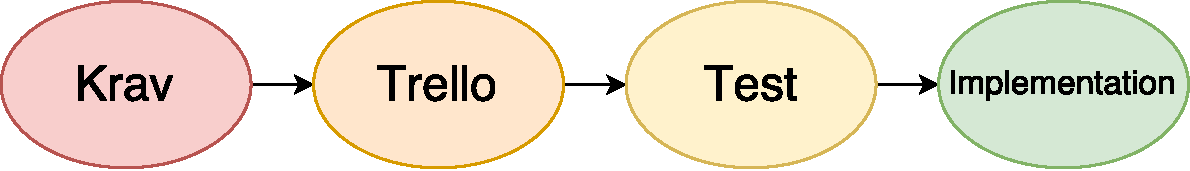
\includegraphics[scale=0.75]{tracability}
\caption{En illustration över arbetets spårbarhet.}
\label{fig:tracability}
\end{center}
\end{figure}
\\
För att uppnå spårbarhet och kunna leverera mot kundens krav har alla Trello-kort en etikett med id för det krav i kravspecifikationen som de implementerar och en beskrivning över de testfall som validerar dess funktionalitet. Se figur \ref{fig:tracability} för en illustration över processen.
I de fall som korten valideras med hjälp av automatiserade tester kommer en lista på testfall som förväntas passera förses, och i de fall manuella tester krävs kommer en detaljerad steg-för-steg-lista förses.
 %Problem reporting and corrective action
\newpage
\section{Verktyg, tekniker och metoder}
Projektgruppen har beslutat om standarder för arbetsverktyg, tekniker och metoder för att underlätta samarbetet. 

\subsection{Trello}
Vi kommer att använda oss av verktyget Trello\cite{website:trello} för att organisera och dela upp arbete i gruppen. 
\\ \\
Varje feature, bugfix och dokumentation blir en issue i Trello som kommer ha en etikett för vilken typ av problem det är, samt en etikett för vilket krav från kravspecifikationen som berörs.

\subsection{GitLab}
Vi använder GitLab\cite{website:gitlab} i samarbete med Linköpings Universitet som värd för båda våra git-repositoryn. I GitLab har vi möjlighet att helt använda git och får dessutom tillgång till några extra funktioner som Slack-integration. 
\\ \\
Källkoden kommer förvaras och versionhanteras på GitLab. Detta betyder att alla kommer jobba mot GitLab när vi delar och versionhanterar den kod vi skriver. Alla branches och merge request ska hänvisa till en eller flera issues i Trello, detta görs genom att koppiera in en länk som pekar på en specifik issue i Trello.
\\ \\
GitLab ska inte användas för att fördela arbete eller för att föra diskussioner om någonting.

\subsection{Google Drive}
Vi använder Google Drive\cite{website:googledrive} för att dela interna dokumenet som enkelt modifieras av alla samtidigt. 
\\ \\
Under möten har sekreteraren mötets dagordning på Google Drive öppet för att lätt följa de anteckningar som skrivs eller refereras till. Google Drive-dokument används även till att dela upp och organisera dokumentskrivandet innan själva praktiska projektet startar, som till exempel denna text.
\\ \\
Google Drive ska inte användas för de ändamål som Trello och GitLab används, utan kompletterar och underlättar för när vi delar interna dokument som inte ska publiceras på något sätt.

 %Tools,techniques and methodologies
\newpage
\section{Kontroll av leverantör}
Projektgruppen har arbetat fram ett dokument Kravspecifikation som innehåller de krav som ställts på applikationen och kommer att jobbas fram i så kallade sprinter eftersom projektet arbetar efter en agil arbetsmetod Scrum \cite{website:scrum}, görs arbetet i sprinter. Efter varje sprint kommer arbetet och kraven revideras av kunden i form av mindre leveranser. %Supplier control(demos)
\newpage
\section{Utbildning}
Internutbildning i gruppen sker antingen individuellt om det rör sig om områden som ingen i gruppen känner att de inte har någon tidigare erfarenhet inom eller de känner att de inte har möjligheten att föra sin erfarenhet vidare. Om en gruppmedlem besitter en erfarenhet som gruppen är i behov av och gruppmedlemen känner sig bekväm i att hålla i en utbildning för resten av gruppen så avsätts tid för det. De utbildningar som gruppen har identifierat och planerat är:
\begin{itemize}
\item \textit{Att skriva testbar kod} - Hålls av utvecklingsansvarig.
\item \textit{Scrum} - Hålls av utvecklingsansvarig.
\item \textit{Komma igång med Git och GitLab} - Hålls av konfigurationsansvarig. 
\end{itemize}
Fler utbildningar kommer att hållas om andra kunskapsbrister hittas eller om viss kunskap behöver fräschas upp, i mån av tid. %Training
\newpage
\section{Riskhantering}
En plan med utförlig beskrivning och förslag på risker och hur riskhantering ska gå till finns att läsa under rubriken Riskhantering i dokmentet Projektplan. %Risk management

\clearpage
\printbibliography

\end{document}